\section{Производительность решения}

Целями следующих экспериментов является выявление эффекта произведенного использованием нескольких глобальных очередей и сопоставлением этих результатов с результатами использования нескольких рантаймов.

\subsection{Ход исследования}

Сценарий предоставленный командой \verb|TATLIN.BACKUP| был использован для измерения пропускной способности системы, состоящей из нескольких рантаймов и одного рантайма с несколькими глобальными очередями, что представлено на рисунке~\ref{fig:tatlin:multi_rt_gp:eval}.

\begin{figure}[H]
    \begin{center}
        \makebox[\textwidth]{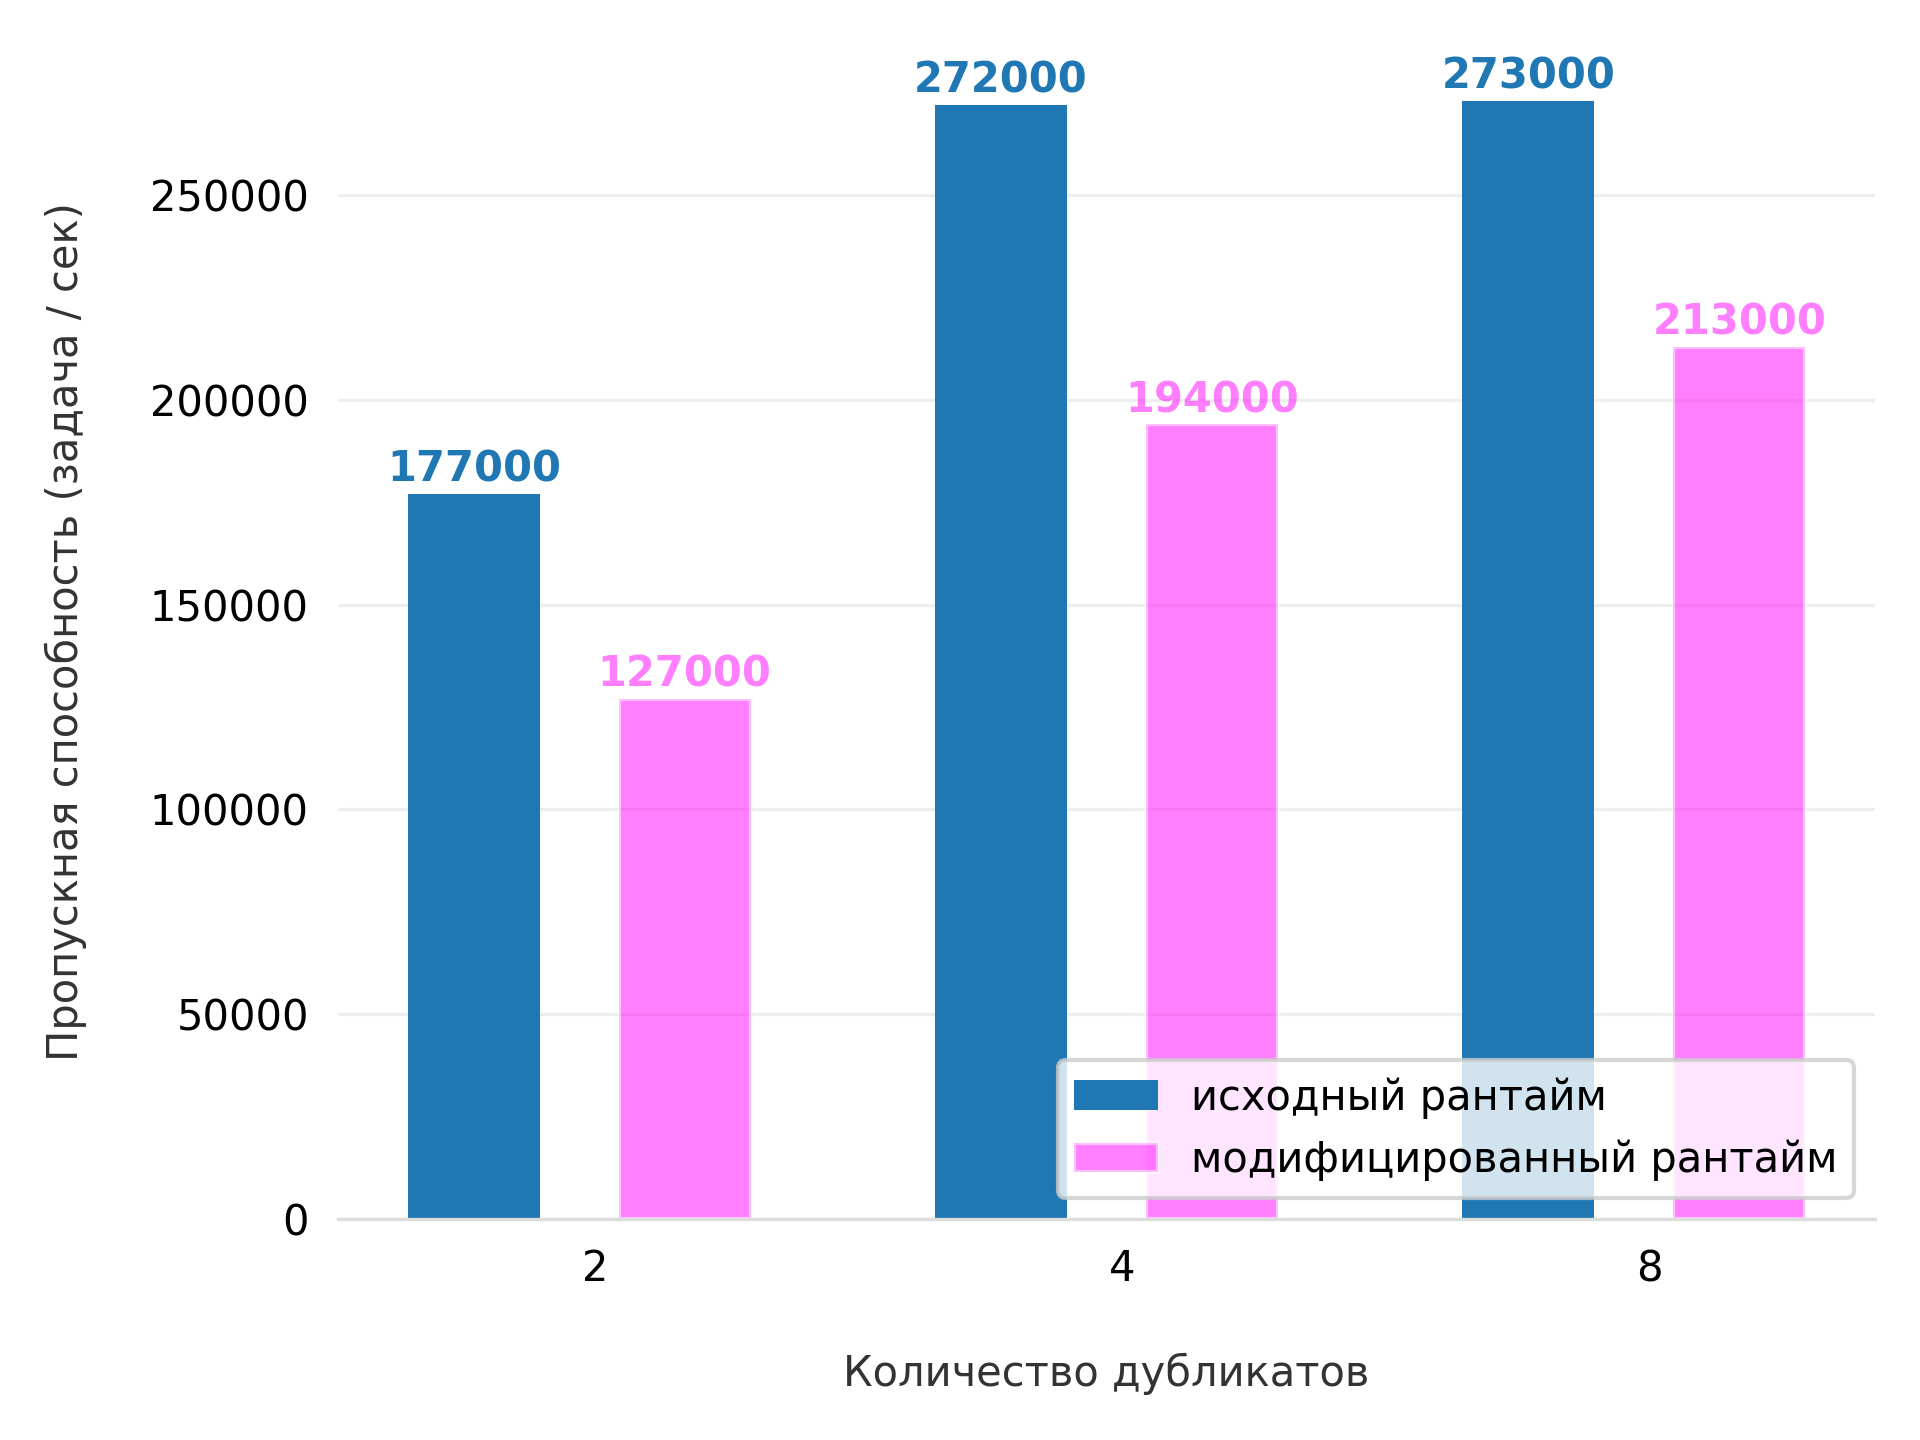
\includegraphics[scale=0.90]{pictures/rt_gp_nsapwner128_nspawn1000.png}}
    \end{center}

    \caption{Производительность системы при использовании нескольких рантаймов.}
    \label{fig:tatlin:multi_rt_gp:eval}
\end{figure}

\subsection{Вывод}

\begin{itemize}
    \item Пропускная способность системы из одного рантайма и одного модифицированного рантайма, содержащего одну глобальную очередь,демонстрируют одинаковую пропускную способность.
    \item При увеличении количества глобальных очередей в системе, состоящей из одного рантайма, наблюдается увеличение пропускной способности. Это ожидаемый результат:
    \begin{itemize}
        \item Меньшее количество воркеров конкурируют за глобальну очередь.
        \item Меньшее количество воркеров пытаются похитить задачи.
    \end{itemize}
    \item Пропускная способность системы, состоящей из одного модифицированного рантайма, содержащего несколько очередей, меньше пропускной способности системы, состоящей из нескольких рантаймов. Это ожидаемый результат --- в системе, состоящей из отдельных рантаймов, требуется меньшее количество синхронизаций:
    \begin{itemize}
        \item Различные метрики, собираемые рантаймом реализованы с помощью атомарных счетчиков, разделяемых в случае одного рантайма.
        \item Многие структуры данных находятся близко в памяти, что может так же требовать дополнительной синхронизации между различными процессорами.
    \end{itemize}
\end{itemize}
